\chapter{Результаты}
\label{ch:results}

\section{Экспериментальная установка}

    Для более точного измерения теплоёмкости твёрдого тела, необходимо уменьшить потери энергии. Для этого в работе использовался калориметр с пенопластовой изоляцией, так как пенопласт является хорошим теплоизолятором. Для увеличения теплоизоляции калориметр также поместили в ящик из многослойной клееной фанеры (см. рис. 1).

    \begin{center}
        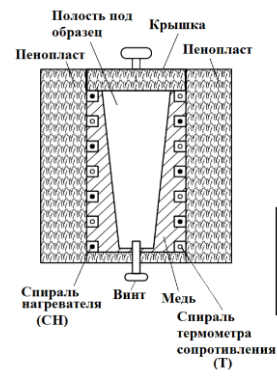
\includegraphics[width=0.5\textwidth]{img/214.png}
    
        Рис. 1. Калориметр с пенопластовой изоляцией, в который встроена спираль нагревателя и термометра сопротивления. Калориметр содержит полость для образца в форме усечённого конуса для более надёжного теплового контакта.
    \end{center}

    
    Внутренние стенки калориметра выполнены из материала с высокой теплопроводностью. Надежность теплового контакта между телом и стенками обеспечивалась их формой: они имели вид усечённых конусов и плотно прилегали друг к другу.
    
    \vspace{1 em}
    
    Экспериментально можно найти зависимость термометра сопротивления от времени при нагревании калориметра с телом при постоянной мощности, зависимость термометра сопротивления от времени при охлаждении калориметра с телом с выключенным нагревателем, зависимость комнатной температуры от времени.

\section{Обработка результатов измерений}

    Измерения проведены для образца из алюминия $m_{\text{алюм}} = (294.1 \pm 0.5)~\text{г}$ и образца из титана $m_{\text{титан}} = (293.2 \pm 0.5)~\text{г}$ (Ход работы см. в Приложении В).

    Полученные данные изображены на графике на рис. 2. 

    \begin{figure}[ht]
        \begin{center}
        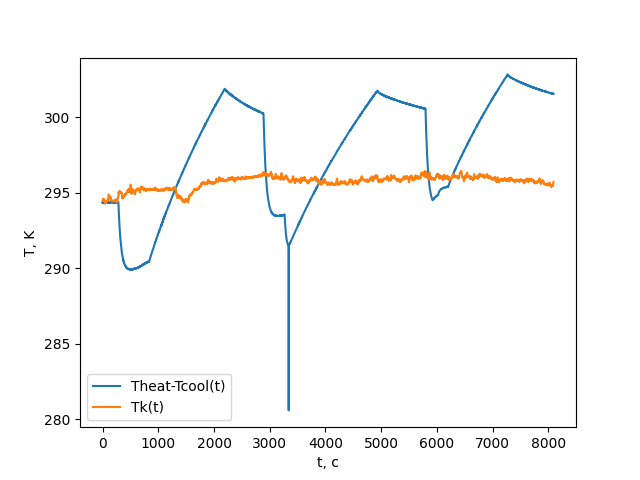
\includegraphics[width=0.75\textwidth]{img/CommonT.png}
        
        Рис. 2. $T_{cool}(t)$ - зависимость температуры от времени при охлаждении, изображена в виде голубой прямой (участки с убывающей температурой).  $T_{heat}(t)$ - зависимость температуры от времени при нагревании, изображена голубой прямой (участки с возрастающей температурой). $T_k(t)$ - зависимость комнатной температуры от времени течение всего эксперимента.         
        \end{center}
    \end{figure}\textbf{}
    
    Из уравнения:
    $$-\frac{C}{\lambda}ln\frac{T_{cool}-T_k}{T-T_k} = t$$
    видно, что отношение $-\frac{\lambda}{C}$ будет равно тангенсу наклона графика в координатах ($t, ln \frac{T_{cool}-T_k}{T-T_k}$).
    
    Построили график зависимости температуры калориметра с телом из алюминия от времени (см рис. 3).
    \begin{figure}[ht]
        \centering
        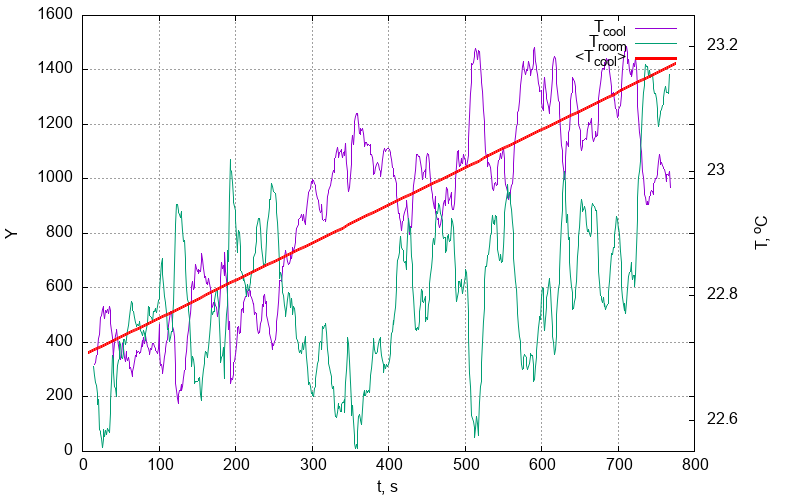
\includegraphics[width=\textwidth]{img/T_cool_2.png}
        \begin{center}
            Рис. 3. График зависимости температуры калориметра с телом из алюминия от времени при нагревании. Фиолетовым и зелёным цветом проведены линии, отображающие зависимость температуры калориметра с телом из алюминия ($T_{cool}$) и комнатной температуры ($T_k$) от времени. Красным цветом проведена прямая, полученная при помощи МНК, которая показывает среднее увеличение температуры системы.  
    \end{center}
    \end{figure}\textbf{}
    
    \FloatBarrier
    Из графика получили $\lambda/C = (1.302\pm0.030)*10^{-4}\textrm{с}^{-1}$

    Подставив это отношение в формулу: $T_{heat}(t) = \frac{P}{\lambda}(1-e^{-\frac{\lambda}{C}t})+T_k$, нашли $\lambda$ для этого случая: $\lambda = 0.118 \pm 0.009$. Затем определили теплоёмкость алюминия, используя теплоёмкость калориметра (нахождение теплоёмкости калориметра см. в Приложении Г):

    $$C_{\sum} = 906.3 \pm 71.6 \, \frac{\textrm{Дж}}{\textrm{К}}, \quad C_{Al} = 247.0 \pm 19.5\, \frac{\textrm{Дж}}{\textrm{К}}, \quad \sigma_{C_{Al}}=7.9\%$$
    $$M_{Al} = 286.9 \pm 0.5\, \textrm{г}, \quad C_{Al} = 860.9 \pm 68.0 \, \frac{\textrm{Дж}}{\textrm{К}\cdot\textrm{кг}}, \quad \sigma_{C_{Al}}=7.9 \% $$

\vspace{1 em}
    
   Построили график зависимости температуры калориметра с телом из титана от времени (см. рис. 4).
    \begin{figure}[ht]
        \centering
        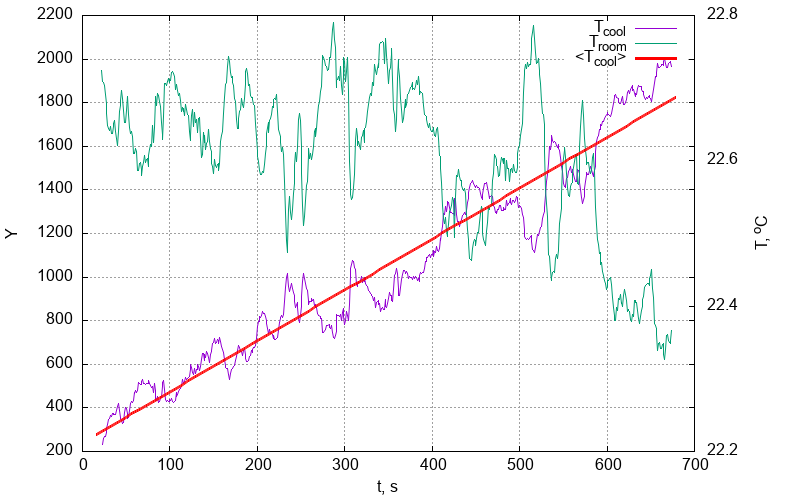
\includegraphics[width=\textwidth]{img/T_cool_3.png}
        \begin{center}
            Рис. 4. График зависимости температуры калориметра с телом из титана от времени при нагревании. Фиолетовым и зелёным цветом проведены линии, отображающие зависимость температуры калориметра с телом из алюминия ($T_{cool}$) и комнатной температуры ($T_k$) от времени. Красным цветом проведена прямая, полученная при помощи МНК, которая показывает среднее увеличение температуры системы.
        \end{center}
    \end{figure}\textbf{}

    
    \FloatBarrier
    Из графика получили $\lambda/C = (2.236\pm0.022)*10^{-4}\textrm{с}^{-1}$. Аналогично, нашли $\lambda = 0.175 \pm 0.012$, а затем опеределили теплоёмкость титана:

    $$C_{\sum} = 818.4 \pm 56.7 \, \frac{\textrm{Дж}}{\textrm{К}}, C_{Ti} = 159.1 \pm 11.0 \, \frac{\textrm{Дж}}{\textrm{К}}, \quad \sigma_{C_{Ti}}=6.9\%$$
    $$M_{Ti} = 290.8 \pm 0.5\, \textrm{г}, \quad C_{Ti} = 547.1 \pm 37.8 \, \frac{\textrm{Дж}}{\textrm{К}\cdot\textrm{кг}}, \quad \sigma_{C_{Ti}}=6.9 \% $$

    \vspace{1 em}

%список литературы отдельно

    Из источника 1 (см. Список литературы) взяли табличные значения удельных теплоёмкостей для алюминия и титана:
    \begin{align*}
        c_{\text{алюм}} &= 0.920~\frac{\text{кДж}}{\text{кг*К}} & c_{\text{титан}} &= 0.530~\frac{\text{кДж}}{\text{кг*К}}
    \end{align*}

    Результаты, полученные в работе, совпали с табличными значениями в пределах погрешностей.

    Большая погрешность результатов объясняется тем, что производилось вычитание теплоёмкости калориметра из суммарной теплоёмкости калориметра и образца. Из-за того, что теплоёмкость калориметра в несколько раз больше получились погрешности порядка $7-8 \%$.